\chapter{Flux Balance Analysis}

The \textbf{Flux Balance Analysis} (FBA) is an analytical technique used to 
study biological systems from a metabolic perspective. The metabolism of a 
system is represented as a set of metabolic reactions, organized in a 
\textit{stoichiometric matrix} that describes these reactions. FBA allows us to 
study the flow of chemical substances through these reactions in the system.

\begin{definition}[\textbf{Metabolic pathway}]
    A \textbf{metabolic pathway} is defined as a sequence (or graph) of 
    metabolic reactions.
\end{definition}

When all metabolic pathways are considered and represented together, we obtain 
the metabolic network (or \textit{metabolome}) of the system, a section of which 
is illustrated in the figure \ref{fig:pathway}.

\begin{figure}[!ht]
    \centering
    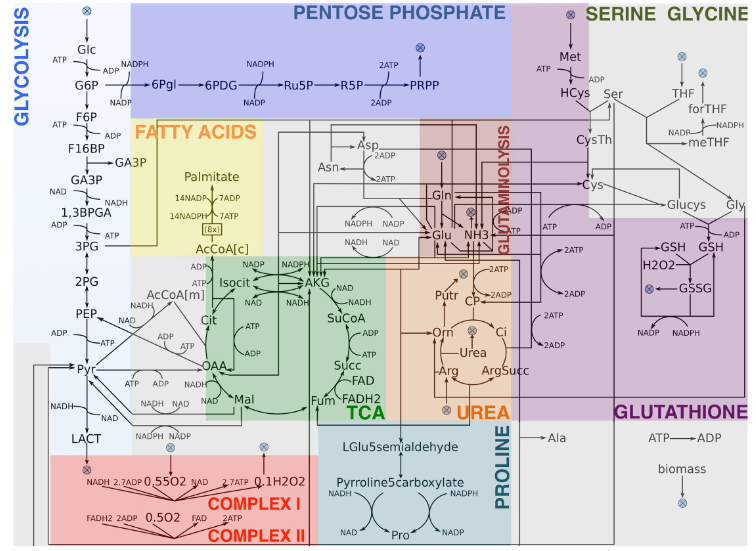
\includegraphics[width=0.5\linewidth]{img/pathway.png}
    \caption{A section of the overall metabolic network of a cell}
    \label{fig:pathway}
\end{figure}

An important aspect to consider when representing biological systems is the level 
of abstraction one wishes to adopt.

The study of cellular metabolism is crucial for understanding numerous diseases, including:
\begin{itemize}
    \item \textbf{cancer}: cancer cells utilize different metabolic pathways from 
        standard ones for energy production, and research focuses on both intracellular 
        metabolism (intra-tumor) and the interactions among cancer cells (inter-tumor);
    \item \textbf{diabetes}
    \item \textbf{obesity}
    \item \textbf{fatty liver disease}
    \item \textbf{Parkinson's disease}
    \item \textbf{Alzheimer's disease}
\end{itemize}

Additionally, metabolism research is fundamental for analyzing the effects of aging, as 
metabolic pathways change over time.

Another reason for studying metabolism is to explore its potential for metabolic engineering.

To identify the most active components within a system, it is useful to analyze metabolic flows. 
In practice:
\begin{itemize}
    \item it is possible to measure the \textbf{metabolome}, i.e., the concentration of metabolites 
        (end products or intermediates of metabolism) at a given time $t$;
    \item the \textbf{fluxome}, or metabolic flows over a time interval $\Delta t$, cannot be 
        directly measured.
\end{itemize}

\begin{definition}[\textbf{Flux}]
In this context, \textbf{flux} is defined as the difference between the rate of “forward” reactions 
and the rate of “reverse” reactions:
\begin{equation}
    \text{flux} = \text{rate}_{forward} - \text{rate}_{backward}
\end{equation}
\end{definition}

\section{Linear Programming}

Several modeling solutions exist to address the challenges of simulating biological systems:
\begin{itemize}
    \item \textbf{Static modeling}
    \item \textbf{Dynamic modeling}
    \item \textbf{Steady-state modeling}: an intermediate approach assuming the system is at 
        equilibrium, allowing simpler analysis.
\end{itemize}

In this context, linear programming is also employed, using:
\begin{itemize}
    \item The \textbf{stoichiometric matrix} $S$, where columns represent reactions and rows 
        represent metabolites;
    \item The \textbf{steady-state condition} expressed as $S \cdot v = 0$;
    \item The \textbf{flux constraints}:
        \begin{equation*}
            v_{min} < v < v_{max}
        \end{equation*}
        which describe different types of flux:
        \begin{itemize}
            \item \textbf{Input fluxes}, regulated by constraints on nutrients;
            \item \textbf{Internal fluxes}, regulated by thermodynamic and reaction 
                rate constraints;
            \item \textbf{Secretion fluxes}, to represent metabolic accumulation, modeling 
                growth and its constraints.
        \end{itemize}
\end{itemize}

Through linear programming, it is possible to calculate the \textbf{area of possible phenotypes}, 
defined by these constraints.

Exchange reactions are characterized by two parameters for reaction $R$, denoted as $R \Longleftrightarrow$:
\begin{itemize}
    \item \textbf{Uptake}: removal from the extracellular environment, or negative flux, 
        ranging from $-\infty$ to $0$;
    \item \textbf{Secretion}: introduction into the extracellular environment, or positive flux, 
        ranging from $0$ to $+\infty$.
\end{itemize}

The process of constraint-based modeling and Flux Balance Analysis (FBA) is as follows:
\begin{itemize}
    \item \textbf{Genome-scale metabolic reconstruction}: analyzing reactions and understanding the 
        pathways of the system;
    \item \textbf{Mathematical representation of metabolic reactions and constraints}, using a 
        stoichiometric matrix $S$, with additional columns for the variables of interest. This matrix is 
        multiplied by the vector 
        \begin{equation*}
            v = \{v_1, \dots, v_n, v_1', \dots, v_m'\}   
        \end{equation*}
        representing reaction flows, yielding $S \cdot v = 0$, a homogeneous linear system in 
        steady-state;
    \item \textbf{Mass balance}: defines a system of linear equations, $S \cdot v = 0$, which 
        represent the constraints of the system to be solved with linear programming;
    \item \textbf{Definition of an objective function} to optimize, of the form:
        \begin{equation}
            z = \sum_i c_i \cdot v_i
        \end{equation}
        where $c_i$ are the weights and $v_i$ are the target coefficients. The function $z$ is used 
        to predict values of interest;
    \item \textbf{Calculation of the optimal flux} that maximizes $z$ through linear programming.
\end{itemize}

Thus, linear programming is used with FBA to ensure flux feasibility, optimize a linear combination 
of the system’s products, and manage boundary conditions.

Naturally, this approach can become computationally complex. The well-known simplex algorithm is 
typically used, which is effective but may exhibit exponential complexity in certain cases.

Usually, using linear programming methods you get an optimal solution, this aspect can be
sometimes limiting. The problem to be faced is essentially that of ranking/choosing the 
different metabolic "states" which emerge in an analysis, when changing, for example, 
parameters or objective function. This kind of talk becomes interesting talking about 
\textbf{metabolic rewiring} (metabolic re-wiring) in the field of cancer.

FBA can be used in many ways, with various applications and extensions. These problems vary 
with the change in weights and objective function, some of them being partly solvable
numerically. All these aspects need to be studied and deepened from time to time.

From the point of view of linear programming, there are several categories of resolvers for 
the continuous case, but we can include them in two macro-categories:
\begin{enumerate}
    \item Solvers based on the simplex algorithm: they work well in most cases even if you 
        have "pathological" cases that make the problem exponential over time; 
    \item Solvers based on internal point methods: unlike solvers based on the simplex
        algorithm, you are guaranteed to find a solution in polynomial time. Unfortunately,
        these methods are difficult to implement.
\end{enumerate}
Besides the continuous case, we also have one in which we introduce integer constraints, 
with variables that belong only to N, thus having the whole linear programming. You can 
also have mixed problem solvers, both continuous and discrete, and these are quite complex 
and sophisticated.
\section{Exploring Fluxes}
During the analysis process we are interested in studying flows. The first step is to 
understand which of all the fluxes we can study are most interesting for us. To do this, 
we start with a complete model (\textbf{Genome Wide Reaction Models}), which is very complex
for the study because it is biologically very realistic and complete, and we proceed to build
a \textbf{Core reaction model}. These models are obtained by simplifying complex models and
grouping reactions, thus obtaining models ready for simulation. In practice, you take a
piece of pathway and ignore the intermediate steps, compacting the representation, simplifying
equations and computational complexity.
\section{Enhanched Growth Model}
We now study the \textbf{ENGRO} model shown in Figure \ref{fig:engro}, which represents the
core model used to represent the growth of a cell. This model has led to the observation that 
cancer cells and many glass-grown cells have a glucose fermentation process, even when there 
is enough oxygen to breathe properly. In other words, instead of fully breathing in the 
presence of an adequate level of oxygen, cancer cells ferment. Currently, it is thought that 
cancer cells ferment glucose while maintaining the same level of respiration that was present 
before the carcinogenesis process, and therefore the Warburg effect would be defined as the 
observation that cancer cells show glycolysis with lactate secretion and mitochondrial 
respiration in the presence of oxygen. 

\begin{figure}[!ht]
    \centering
    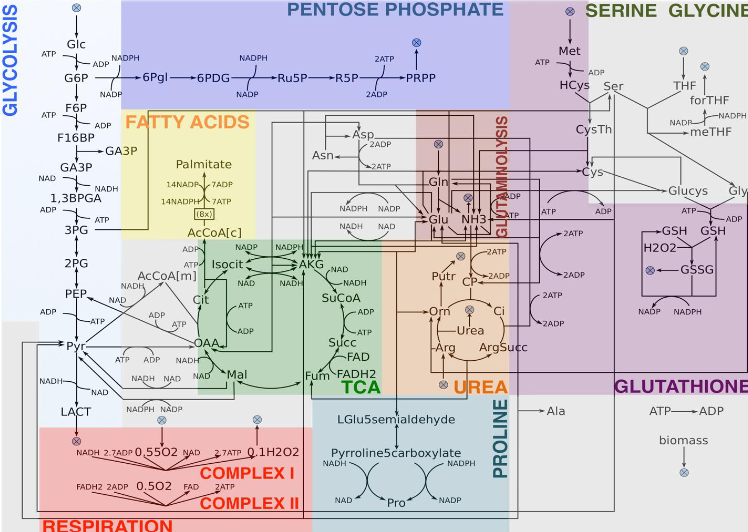
\includegraphics[width=0.5\linewidth]{img/ENGRO.png}
    \caption{Modello ENGRO}
    \label{fig:engro}
\end{figure}

To study this system, we did not limit ourselves to a single objective function of linear 
programming, but studied several, having in fact a meta-programming problem. The entire space
of the FBA solutions is then studied, as well as how a model can be \textbf{perturb} and again used to analyse the perturbation.

The first step is to analyse the results obtained with FBA. For example, if one wants to look
for the optimal value of the growth rate in function of the availability of nutrients entering 
the system one can start by noting that when the amount of glucose drops a greater quantity of 
oxygen is required and vice versa.

An initial study that can be carried out with the ENGRO model is therefore to place certain 
constraints on substances entering the system, or to place constraints on certain flows. This 
is done to study, in the light of a certain objective function, the optimal distribution of 
flows. In particular, we will see which of these are up-regulated and which down-regulated.
Obviously, the optimal solutions can be different, it is therefore a good rule to explore the 
whole space of acceptable solutions, varying the various weights of the objective function 
etc$\dots$, also making certain reactions enable/disable from time to time.

Consider, for example, the following conditions on the set of solutions and on a number $j$ of 
interactions:
\begin{equation}
    \begin{split}
        \sum_{i \in NZ_{j - 1}} y_i \geq 1 \\
        \sum_{i \in NZ_j} w_i \leq |NZ_k|-1 \, \, \, \text{for} \,\,\,k = 1, 2, \dots j - 1\\
        y_1 + w_i \leq 1, \,\, \forall i \\ \alpha \cdot w_i \leq v_i \leq \beta \cdot w_i \, \, \forall i
    \end{split}
\end{equation}
At each iteration $j$, at least one of the non-zero flows from the previous solution, namely 
$NZ_{j - 1}$, shall be set to zero, where the binary variable $y_i$ is 1 if that fluxe is 
selected to be removed from base at iteration $j$. The binary variable $w_i$ is then forced to 
zero if $y_i$ is one, and the upper and lower bounds for that particular stream are then bound 
to zero.

The equations ensure that alternative bases are not revisited by removing at least one non-
zero variable found in previous iterations. This is therefore a recursive algorithm for the 
calculation of alternative optimals using mixed integer linear programming (MILP) and allows 
us to enumerate the various alternative solutions.

Another interesting thing to study is how the phenotype changes as certain disturbances in the
system vary. To do this, we then start with a wild-type phenotype and apply various changes to 
it in order to obtain a modified phenotype. The following disturbances can be applied to 
obtain this result: (\textit{i}) nutrient disturbances, (\textit{ii}) gene deletion.
In addition, other tests may be performed less frequently, such as: (\textit{i}) deletion of
reactions, (\textit{ii}) thermal shock.

From the most modelling/mathematical point of view, there are various ways of studying the 
disturbance of the system. A first approach is to use simply the FBA, simulating metabolic 
responses, for example by studying knockouts (which could be multiple in the system under 
analysis) and nutrient variation. Let us take an example where, in the wild-type case, we want 
to maximize growth. There is thus a certain objective function with certain constraints, such 
as:
\begin{equation}
  \begin{array}{rrclcl}
    \displaystyle \max & f_{growth} \\
    \textrm{s.t.} & b_L & \leq & f & \leq b_{U} \\
                       & Sf & = & [0] \\
  \end{array}
\end{equation}
We can add constraints to obtain:
\begin{equation}
  \begin{array}{rrclcl}
    \displaystyle \max & f_{growth} \\
    \textrm{s.t.} & b_L & \leq & f & \leq b_{U} \\
                    & Sf & = & [0] \\
                    & b_L & \leq & f_{mut} & \leq b_{U} \\
  \end{array}
\end{equation}

The added constraints can be used to represent one of the above listed disturbances.

However, there are still some limitations:
\begin{itemize}
    \item The mutation may not grow optimally if natural selection has not had a chance to act on the new genetic background;
    \item has "only" found an excellent alternative, having however, from the point of view of linear programming, solutions that are located on the vertices;
\end{itemize}
This procedure is however usually automated, perhaps using a list of genes to be activated/
deactivated, keeping track of each change and the variation in results obtained through it.

Overcoming the classical approach, the first step is to introduce a particular biological 
hypothesis, called the Minimization of Metabolic Adjustment (MOMA) hypothesis, which assumes 
that a mutation will tend to approximate when it has the wild-type as much as possible. More 
formally a MOMA flow vector with minimum euclidean distance from a single optimal wild-type 
entity is found, subject to the constraints of the mutation. There is thus a certain objective 
function with certain constraints, such as:
\begin{equation}
  \begin{array}{rrclcl}
    \displaystyle \max & f_{growth} \\
    \textrm{s.t.} & b_L & \leq & f & \leq b_{U} \\
                    & Sf & = & [0] \\
  \end{array}
\end{equation}
using MOMA:
\begin{equation}
  \begin{array}{rrclcl}
    \displaystyle \min & |m -f_{opt}| \\
    \textrm{s.t.} & b_L & \leq & f & \leq b_U \\
                    & S_m & = & [0] \\
                    & b_L \leq f_{mut} \leq b_U
  \end{array}
\end{equation}

Thus obtaining not an excellent on a summit but the closest solution, under the MOMA hypothesis. Obviously, there are limitations here too:
\begin{itemize}
    \item the MOMA hypothesis will push the metabolism in the mutant towards the arbitrary distribution of single optimal flow obtained with the FBA but there are still alternative solutions that maximize growth and other sub-optimal solutions
    \item growth is not assured in the mutations
\end{itemize}

Another approach is the more probabilistic one, based on a random sampling of the various 
parameters of linear programming. There are therefore two types of sampling approach:
\begin{itemize}
    \item \textbf{Hit-and-Run} (HR), where you have uniform sampling within the region of the
        allowed solutions, that is a valid initial point is moved repeatedly into space
        according to probabilistic rules. An objective function of the type is obtained by
        having a random pair of reactions:
        \begin{equation*}
            F = w_i \cdot f_i + w_j \cdot f_j
        \end{equation*}
    \item \textbf{Convex Basis} (CB) where the simplex algorithm is used with a random set of
        objective functions to be maximized. Maximising each of these objective functions will
        give a corner in the space of solutions.
\end{itemize}
Obviously the number of combinations that can be obtained with sampling can be really huge so
it must be carried out "under control".

Another interesting element is the so-called ENGRO \textbf{Z-score}. Such value other does not
measure the difference between mutation and wild-type entity, by measuring on wild-type means
and standard deviation:
\begin{equation}
    Z = \frac{\overline{X}_1 - \overline{X}_2}{\sqrt{\frac{\sigma^2_1}{n} + \frac{\sigma^2_2}{n}}}
\end{equation}
Having therefore a high value for Z corresponds to a high difference between the wild-type 
entity and the mutation.
\section{Guiding the Search}
The current study of FBA-based methods has several limitations, although some extensions have 
been created to overcome them. Among the various limitations we have:
\begin{itemize}
    \item Is based on the assumption of steady-state, leading to difficulties in studying the
        dynamics of the system
    \item does not provide any information on the concentrations of metabolites
    \item Requires limited choice of objective function
    \item has a limit in predicting the net behaviour, or the sum of flows, of possibly 
        heterogeneous cells within a population.
\end{itemize} 

It was also asked whether the metabolism works only to maximise the growth rate. There is
evidence, studied in the laboratory, that the deletion of some metabolic genes cause an 
increase in growth rates and biomass yield compared to the wild-type entity. The selective 
pressure to increase growth rate must be balanced by other demands on metabolism, such as 
cellular maintenance or sensory apparatus, reducing growth rate in favor of overall fitness. 
Also, limitations of evolutionary time and genetic variability may mean that metabolism is not 
optimal for any target, so we cannot necessarily exclude from consideration the many flow 
configurations that support, for example, $90\%$  (but also percentages) of maximum growth.
These support configurations are useful when deciding linear programming constraints.

The key point of the speech is that perhaps with an optimal solution from the point of view 
of the growth rate it leads to maximize biomass while with a sub-optimal solution, always side 
growth rate, you get not only an acceptable biomass but maybe also, For example, the 
production of other components, perhaps biofuels.
\section{Metabolic Pathways Rewiring}
We can see cancer as a "stochastic disease", resulting from a series of mutations affecting the 
cells of our body and involving the selection of a phenotype useful solely for its own purposes. 
Cancer cells are therefore, roughly speaking, part of normal cell sets that have accumulated a 
random set of mutations and epigenetic modifications. It is therefore that the cellular evolution 
has been in these cases somewhat modified and then we can study the normal functioning of metabolism, 
this sort of "metabolic wiring" ("metabolic connection") of those sets that have generic properties 
which statistically correspond to the real cell properties. 

In more mathematical terms we recognize the area of feasibility through linear programming. Outside of 
this area you have the impossible phenotypes while inside you have all the phenotypes possible, where 
various subsets with similar properties can be identified. The metabolism is therefore assumed to be 
similar between normal and carcinogenic cells, but if does a different study through the FBA.

To explore the space of possible "links" we proceed by random sampling of weights, changing objective 
function each time, and also sampling reactions, aiming finally to maximize the sum of the flows through 
certain reactions. The flow distributions obtained may be an efficient representation of a randomly 
mutated cell population. 

After making various analyses through the FBA, sets of different metabolic responses to disturbances 
are created and a sort of binary tree is created, which is divided according to the success rates of 
certain actions. From this tree, different information can be obtained on the system, since the different 
branches allow us to distinguish normal behaviour from carcinogenic behaviour.